\documentclass[11pt]{amsart}
\usepackage{amsmath,amsthm, amscd, amssymb, amsfonts, mathtools,color}
%\usepackage{tabu}
\usepackage[all]{xy}
\usepackage{mathrsfs}
\usepackage{enumitem}
\usepackage[T2A,T1]{fontenc}
%\usepackage{rotating}
\usepackage{multicol}
\newcommand{\pinom}{\genfrac{[}{]}{0pt}{}}
\usepackage{hyperref}

\allowdisplaybreaks

%\usepackage[basic,optics]{circ}
%\usepackage[spanish]{babel}
\usepackage[ansinew]{inputenc}
\usepackage{graphicx,fancyhdr}

%\usepackage[dvips, dvipsnames, usenames]{color}
\newcommand{\com}[1]{\textcolor{blue}{\textbf{#1}}}
\newcommand{\diag}{\operatorname{diag}}



\newcommand{\pre}{\mathfrak{Pre}}
\newcommand{\pref}{\mathfrak{Pre}_\textrm{fGK}}

\newcommand{\post}{\mathfrak{Post}}
\newcommand{\postf}{\mathfrak{Post}_{\textrm{fGK}}}

\newcommand{\deriv}{\mathfrak d}
\newcommand{\derv}{\mathfrak D}

\newcommand{\Lie}{\operatorname{Lie}}

\newcommand{\nucleo}{\mathbf R}
\newcommand{\Nuc}{\mathcal O}
\newcommand{\gen}{\mathbf{g}}
\newcommand{\Gb}{\mathbf G}
\newcommand{\Hb}{\mathbf H}
\newcommand{\Bb}{\mathbf B}
\newcommand{\uno}{{\mathbf 1}}

\newcommand{\ya}{\mbox{\usefont{T2A}{\rmdefault}{m}{n}\cyrya}}
\newcommand{\zh}{\bx}%{\mbox{\usefont{T2A}{\rmdefault}{m}{n}\cyrzh}}
\newcommand{\Zh}{\mathbb X}%{\mbox{\usefont{T2A}{\rmdefault}{m}{n}\CYRZH}}


\newcommand{\supp}{\operatorname{supp}}
\newcommand{\verma}{M}

\newcommand{\hopfuno}{\mathtt{H}}
\newcommand{\hopfdos}{\mathtt{K}}
\newcommand{\hopfdouble}{\mathtt{D}}
\newcommand{\xb}{x}%{\mathbf x}
\newcommand{\ub}{u}%{\mathbf u}


\numberwithin{equation}{section}
\newtheorem{theorem}{Theorem}[section]
\newtheorem{lemma}[theorem]{Lemma}
\newtheorem{coro}[theorem]{Corollary}
\newtheorem{conjecture}[theorem]{Conjecture}
\newtheorem{prop}[theorem]{Proposition}
\newtheorem{claim}{Claim}[section]

\newtheorem{paso}{Step}

\theoremstyle{definition}
\newtheorem{definition}[theorem]{Definition}
\newtheorem{example}[theorem]{Example}
\newtheorem{question}{Question}
\newtheorem{problem}{Problem}
\newtheorem*{strategy}{Strategy}
\newtheorem{notation}{Notation}


\newtheorem{xca}[theorem]{Exercise}
\theoremstyle{remark}
\newtheorem{remark}[theorem]{Remark}

\newtheorem{step}{Case}
\newtheorem{case}{Case}
\newtheorem{caso}{Step}
\newtheorem{posi}{}[caso]

\newtheorem{caso2}{Step}
\newtheorem{posic}{}[caso2]

\newcommand{\pf}{\begin{proof}}
\newcommand{\epf}{\end{proof}}

\newcommand{\sfm}{\mathsf{m}}
\newcommand{\sfM}{\mathsf{M}}
\newcommand{\sfr}{\mathsf{r}}
\newcommand{\sfs}{\mathsf{s}}
\newcommand{\sft}{\mathsf{t}}
\newcommand{\sfu}{\mathsf{u}}
\newcommand{\sfW}{\mathsf{W}}
\newcommand{\sfy}{\mathsf{y}}
\newcommand{\y}[2]{\sfy_{#1}^{(#2)}}

\newcommand{\lu}{\mathcal{L}}
\newcommand{\luq}{\lu_{\bq}}
\newcommand{\fO}{\mathfrak O}
\newcommand{\spl}{\mathfrak{sl}}

\newcommand{\fjdos}{\hspace{-1pt}j + \frac{1}{2}}
\newcommand{\fkdos}{\hspace{-1pt}k + \frac{1}{2}}

\newcommand{\fudos}{\hspace{-1pt}\frac{3}{2}}
\newcommand{\fdos}{\tfrac{3}{2}}
\newcommand{\futres}{\hspace{-1pt}\frac{5}{2}}
\newcommand{\ftres}{\tfrac{5}{2}}
\newcommand{\inc}{\mathscr{I}}

%Itemize
\newcommand{\vi}{\textbf{(i)} }
\newcommand{\vii}{\textbf{(ii)} }
\newcommand{\viii}{\textbf{(iii)} }
\newcommand{\viv}{\textbf{(iv)} }
\newcommand{\vv}{\textbf{(v)} }
\newcommand{\vvi}{\textbf{(vi)} }
\newcommand{\vvii}{\textbf{(vii)} }
\newcommand{\vviii}{\textbf{(viii)} }
\newcommand{\vix}{\textbf{(ix)} }
\newcommand{\vx}{\textbf{(x)} }
%-----------------------------------------------------

%Letters
\newcommand{\ba}{ \mathbf{a}}
\newcommand{\kk}{ \mathbf{k}}
\newcommand{\ku}{ \Bbbk}
\newcommand{\fp}{\mathbb F_p}

\newcommand{\kut}{ \ku^{\times}}
\newcommand{\Ck}{\mathbb C}
\newcommand{\G}{\mathbb G}
\newcommand{\gb}{\mathbf g}
\newcommand{\ghost}{\mathscr{G}}
\newcommand{\as}{\mathtt{a}}
\newcommand{\qmb}{\mathtt{q}}
\newcommand{\x}{\mathtt{x}}
\newcommand{\yt}{\mathtt{y}}

\newcommand{\wtoba}{\widetilde{\toba}}
\newcommand{\ttoba}{\widetilde{\mathfrak B}}


\newcommand{\I}{\mathbb I}
\newcommand{\Iw}{\mathbb I^{\dagger}}
\newcommand{\idd}{\mathbb I^{\ddagger}}
\newcommand{\J}{\mathbb J}
\newcommand{\N}{\mathbb N}
\newcommand{\bn}{\mathbf n}
\newcommand{\bp}{\mathbf{p}}
\newcommand{\bq}{\mathbf{q}}
\newcommand{\bx}{\mathbf{x}}
\newcommand{\Sb}{\mathbb S}
\newcommand{\Q}{\mathbb Q}
\newcommand{\Uu}{\mathbb U}
\newcommand{\V}{\mathbb V}
\newcommand{\Vb}{\mathbb V_{\text{block}}}
\newcommand{\Vs}{\mathbb V_{\text{ss}}}
\newcommand{\Z}{\mathbb Z}
\newcommand{\zt}{\Z^{\zeta}}

\renewcommand{\_}[1]{_{\left( #1 \right)}}
\renewcommand{\^}[1]{^{\left( #1 \right)}}

\newcommand{\sx}{\mathsf{x}}
\newcommand{\tx}{\mathtt{x}}
\newcommand{\tz}{\mathtt{z}}
\newcommand{\sy}{\mathsf{y}}
\newcommand{\cA}{\mathcal{A}}
\newcommand{\cB}{\mathcal{B}}
\newcommand{\cO}{\mathcal{O}}
\newcommand{\cE}{\mathcal{E}}
\newcommand{\cF}{\mathcal{F}}
\newcommand{\cBt}{\widetilde{\mathcal{B}}}
\newcommand{\dpn}{\widetilde{\mathcal{B}}}
\newcommand{\cC}{\mathcal{C}}
\newcommand{\Cf}{\cC_{\text{GK-f}}}
\newcommand{\D}{\mathcal{D}}
\newcommand{\cU}{\mathcal{U}}
\newcommand{\E}{\mathcal{E}}
\newcommand{\cH}{\mathcal{H}}
\newcommand{\cI}{\mathcal{I}}
\newcommand{\cJ}{\mathcal{J}}
\newcommand{\cL}{\mathcal{L}}
\newcommand{\Pc}{{\mathcal P}}
\newcommand{\cR}{\mathcal{R}}
\newcommand{\Ss}{{\mathcal S}}
\newcommand{\T}{\mathcal{T}}
\newcommand{\cV}{\mathcal{V}}
\newcommand{\X}{\mathcal{X}}
\newcommand{\Xf}{\X_{\text{fin}}}
\newcommand{\Xif}{\X_{\infty}}
\newcommand{\JJ}{\mathcal{J}}


\newcommand{\g}{\mathfrak g}
\newcommand{\kh}{\mathfrak h}
\newcommand{\ngo}{\mathfrak n}
\newcommand{\Ug}{\mathfrak U}
\newcommand{\Fg}{\mathfrak F}

\newcommand{\lstr}{\mathfrak L}
\newcommand{\cyc}{\mathfrak C}
\newcommand{\pos}{\mathfrak P}

%------------------------------------------------------

%Operatorname
\newcommand{\ad}{\operatorname{ad}}
\newcommand{\Alg}{\Hom_{\text{alg}}}
\newcommand{\Aut}{\operatorname{Aut}}
\newcommand{\Frac}{\operatorname{Frac}}
\newcommand{\AuH}{\Aut_{\text{Hopf}}}
\newcommand{\coker}{\operatorname{coker}}
\newcommand{\car}{\operatorname{char}}
\newcommand{\Der}{\operatorname{Der}}
\newcommand{\End}{\operatorname{End}}
\newcommand{\id}{\operatorname{id}}
\newcommand{\gr}{\operatorname{gr}}
\newcommand{\GK}{\operatorname{GKdim}}
\newcommand{\Hom}{\operatorname{Hom}}
\newcommand{\ord}{\operatorname{ord}}
\newcommand{\rk}{\operatorname{rk}}
\newcommand{\soc}{\operatorname{soc}}
\newcommand{\Obj}{\operatorname{Obj}}
\newcommand\Char{\operatorname{char}}
\newcommand{\Svec}{\operatorname{\textsf{sVec}}}
\newcommand{\svec}{\operatorname{\textsf{svec}}}
\newcommand{\vect}{\operatorname{Vec}}
\newcommand{\srep}{\operatorname{\textsf{sRep}}}
\newcommand{\ev}{\operatorname{ev}}
\newcommand{\evt}{\widetilde{\operatorname{ev}}}
\newcommand{\coev}{\operatorname{coev}}
\newcommand{\coevt}{\widetilde{\operatorname{coev}}}
\newcommand{\sTr}{\operatorname{sTr}_q}
\newcommand{\sTrNormal}{\operatorname{sTr}}
\newcommand{\Tr}{\operatorname{Tr}}
\newcommand{\Irr}{\operatorname{irrep}}
\newcommand{\IRR}{\operatorname{Irrep}}
\newcommand{\Ind}{\operatorname{Ind}}
\newcommand{\Res}{\operatorname{Res}}
%------------------------------------------------------

%Others
\newcommand{\doble}{\mathfrak d}
\newcommand{\Bdiag}{\mathcal{B}^\mathrm{diag}}
\newcommand{\Vdiag}{\cV^\mathrm{diag}}
\newcommand{\toba}{\mathscr{B}}
\newcommand{\Ds}{\mathscr{D}}
\newcommand{\ot}{\otimes}
\newcommand{\realroots }{\boldsymbol{\Delta }^{\mathrm{re}}}
\newcommand{\roots }{\boldsymbol{\Delta }}
\newcommand{\siderem}[1]{$^{(*)}$\marginpar{#1}}

\newcommand{\yd}[1]{{}^{ #1 }_{ #1 }\mathcal{YD}}
\newcommand{\dy}[1]{\mathcal{YD}^{ #1 }_{ #1 }}
\newcommand{\lmod}[1]{{}_{ #1 }\mathcal{M}}

\DeclareRobustCommand{\stirling}{\genfrac []{0pt}{}}
\DeclareRobustCommand{\stirlingtwo}{\genfrac \{\}{0pt}{}}
\newcommand{\rightarrowdbl}{\rightarrow\mathrel{\mkern-14mu}\rightarrow}

\newcommand{\xrightarrowdbl}[2][]{%
\xrightarrow[#1]{#2}\mathrel{\mkern-14mu}\rightarrow
}

\newcounter{tabla}\stepcounter{tabla}
\renewcommand{\thetabla}{\Roman{tabla}}

%\DeclarePairedDelimiter\ceil{\lceil}{\rceil}
%\DeclarePairedDelimiter\lfloor{\lfloor}{\rfloor}

\begin{document}
\noindent
\title[The Noether protocol]
{The Noether protocol}
%\author[Pe\~na Pollastri]
%{H\'ector Pe\~na Pollastri}








\maketitle

\begin{abstract}
	The Noether Protocol is a decentralized protocol designed to harvest the idle computing power of casual PC users and tokenize it in order to empower the scientific communities of LATAM. 
	
	Any user can lend its idle processing power to the protocol through the Cardano blockchain and earn NOETH tokens using a regular CPU. This token harvests a pre-existing and wasted value. It will be needed to access the protocol open infrastructure for distributed computing. 
	
	Our goal is to create a decentralized market of computing power that allows private purchase at competitive prices but, at the same time, favors scientific endeavors. The protocol achieves this through a complex distribution and emission algorithm built by scientists for scientists. 
	
\end{abstract}
\section{Introduction}
Most casual PC users spend an average of 20\% of their CPUs theoretical computing power. This is a result of the advancement of multicore, multithreading technology, where the bottlenecks in performance are mainly linked to the memory wall problem, not to the CPUs computing power. Many users have stalled and idle cores that play no role in their day-to-day work. A structural phenomenon that can be traced back to the CPU computing race, a race that has no reflection in the actual computing power spent by the general public.

But this computing power is an extremely valuable resource for the scientific community, and particularly to scientists who work in developing countries. CPUs and GPUs increasing prices have a major impact on developing countries, where most scientists' purchasing power is limited by weak currencies and poor economies. A fact that is magnified by the sky-rocketing prices of these products that cryptocurrency mining aggravates.

This scenario implies a constant wasted potential on idle processors that could be gathered and capitalized by the scientific community and by private investors. The Noether Protocol addresses this phenomenon through a specific protocol based on a token that rewards PC users in exchange for their idle computing power: the NOETH token. 

Inspired by the work of Emmy Noether, renowned mathematician, the NOETH token incentivizes PC users to volunteer their idle processing power. This power is harnessed by The Noether Protocol and assigned to projects that need it in accordance with a rigorous distribution algorithm. The process distributes pre-existing value, and consequently the decentralized wealth (created by the users and beneficiaries of the Noether Protocol) fuels the NOETH token price.

%\section{Our team} The team behind The Noether Protocol includes physicists, mathematicians, computer scientists and experts in cryptocurrencies, as well as lawyers and software developers, to ensure a safe and serious experience, akin to those who identify themselves with the Cardano Ecosystem and its core values.

\section{How does it work?}

The Noether Protocol adapts the middleware BOINC to the crypto space. This software gathers CPU and GPU cycles to perform distributed computing through the completion of {\bf tasks}. 


These tasks are mathematical problems that can be computed independently. This is how parallel computing works but, in this case, the computing doesn't need to be performed in the same physical machine. In this sense, a distributed system has different components that interact with one another to archive a common goal, and this creates a cooperative network.

BOINC currently has over 5 million users. SETI@home, the project that analyzes radio signals to find signs of extraterrestrial intelligence, runs through this middleware.

The protocol is built within the infrastructure of this proven open software. But there are key differences between most BOINC-based projects and The Noether Protocol:

\begin{itemize}
\item Our protocol will offer a concrete reward, the NOETH token, that will encourage PC users to volunteer their processing power, and it will be easier to promote projects on our platform due to its decentralized nature.
	
\item Most projects built upon the BOINC open software originated in developed and rich countries, whose scientific communities do not have to face the same obstacles that scientists in third-world countries endure on a daily basis. This is a core feature in The Noether Protocol's identity.

\item The NOETH token can be used to purchase proccessing power in a descentralized manner. This utility adds value to the token and will attract private investors that can access said computing power at competitive prices, a fact that will strengthen the network and its incentives.

\item  The Noether Protocol, unlike any other BOINC-based project, is tailored to the specificities and idiosyncrasies of the crypto environment. It is designed to run on the Cardano blockchain and to benefit from its unlimited potential.  
\end{itemize}
Regular PC users can download a customized BOINC client and lend their processing power in order to mint NOETH tokens that are distributed to Cardano-based wallets. This computing power can be purchased with NOETH tokens by private investors, but the emission algorithm ensures that scientific institutions receive a fraction of all the minted tokens without any cost, giving them priority on the processing power pool. 

This process involves an emission algorithm that takes into account the processing power lent by any given user on a Cardano epoch and offers a proportional reward in NOETH tokens. These tokens can be claimed in accordance with the criteria of the distribution algorithm, which also rewards scientific institutions in LATAM to give them priority on the processing power pool and contemplates a communal treasury.  

\section{Why fund science in developing countries?}
Most developing countries cannot afford significant scientific funding, for this is an area where results are not immediately shown. We live in countries where urgent matters tend to sideline fundamental necessities such as scientific research. This ends up causing a great asymmetry between the scientific talent of developing countries (mysteriously born in any remote corner of the world) and the resources available to take advantage of these exceptional professionals.

Many great scientists fail to fulfill their potential due to a lack of proper tools and resources. This is a real world problem. Let's remember that computing power is essential to scientific endeavors such as molecular biology, protein folding studies, oncological research, epidemiological simulations, etc.

If the blockchain applications become merely speculative projects without any real utility, we will be wasting this powerful technology. And we believe that science funding in developing countries is a project faithful to Cardano's core values: a serious ecosystem that aims to solve real problems.

\section{The NOETH token}

The NOETH token has all the advantages of any cryptocurrency: decentralization, security and a revolutionary technology in terms of value exchange and storage. It's also censorship resistant, and this is decisive in the scientific field.

Additionally, our project is dealing with pre-existing value: the wasted processing power of idle cores. Redistributing this asset is a source of value in and of itself. The users do not necessarily have to be involved in any scientific community in particular, for they will be rewarded anyway in exchange for their idle processors.

The BOINC client will compute how many tasks the user is clearing and how much computing power is being volunteered to the grid, and will award such a user a proportional amount of NOETH.

The token is distributed in Cardano epochs, and the amount of tokens minted in each epoch depends on the quantity of lending users.
We cannot have a max supply, for once the last NOETH token is minted, there would be no incentive to sustain the grid. So, in order to protect the token's value, the quantity of tokens awarded will be controlled by a logarithmic-like function. That is: a function that grows without bounds, but its rate of growth tends to zero. The NOETH token will be deflationary, for this function will create not a theoretical max supply, but a practical one.

\section{Why launch on Cardano?}

Crypto's scene, nowadays, seems full of schemes trying to make a quick buck straight out of people's expectations. But in science there is no rush. Or rather, rush is counterproductive to the scientific task. And in a world dominated by speed, fuss and at times even irrationality, the value of Cardano's slow, conscientious and professional stride cannot be overstated.

The Noether Protocol is a project built by scientists, inspired by scientists and most importantly: for scientists. So what better chain than Cardano to bring it to life? Cardano is the only project that, since its conception, has always put trusted science above quick and unstable results. Is the project that for many years had to carry the burden of this serious and professional decision in the midst of scams and pump and dump strategies.


Climate awareness also plays an important role in this decision. Any project within the Cardano ecosystem can boast the advantages of Proof of Stake (PoS) over Proof of Work (PoW) in terms of ecological consciousness in a world that is increasingly concerned about the carbon footprint that we produce in our daily activities.

It is known that major PoW projects have a polluting network that wastes immense amounts of computing power. PoS blockchains are designed precisely to correct this unnecessary excess. 

In addition, our protocol aims to recapture all that wasted potential in order to redirect it to projects with real life utilities. Not just infinite mathematical calculations to protect blockchains that can be secured through other, more sophisticated methods. That power can help instead scientists that investigate pandemics, cures diseases or even actively combat climate change itself.



\section{Tokenomics}

The NOETH token is distributed in accordance to Cardano epochs plus an initial emission before the project is launched. Then we enumerate the epochs $n=1,2,\dots$ with natural numbers, where epoch $1$ coincides with the project launching. Initially, there are $\kappa_0 = 10000$ tokens distributed before the automatic emission system takes place. These are distributed as follows:
\begin{itemize}
	\item $40\%$  given to scientific institutions, including universities, research centers, etc.
	\item $30\%$    distributed through \emph{airdrops} to early adopters that follow the project in social media.
	\item $20\%$   destined for the developing team.
	\item $5\%$    saved as a treasury.
	\item $5\%$   for future collaborations.
\end{itemize}



Afterwards, for the epoch $n\in\N$ we distribute a certain quantity of tokens $\kappa_n$. Hence we have a function $\kappa\colon \N \longrightarrow \mathbb{R}$ called \emph{the emission function}. Clearly $\kappa$ depends of the epoch $n$, but it also dependant on the demand of the token. To measure this variable we need the following definition.


\begin{definition}
	For each epoch $n$, we define the \emph{heat of the network} $h_n$ as how many users lent their computing power in said epoch.
\end{definition}

%This concept measures how big the demand of the token is, and the emission rate will depend of this variable. 
Now, let $\kappa_n$ be defined recursively as follows:

\begin{align*}
\kappa_{n+1} = \kappa_n \times \mathcal{H}_n+ \frac{100\times (1+ h_n)}{n},
\end{align*}

where 
\begin{align*}
\mathcal{H}_n = \begin{cases*}
\frac{1}{2}& \text{ if } 72| n\\
1 & \text{ otherwise}.
\end{cases*}
\end{align*}
The number $72$ is chosen because that is the number of Cardano epochs needed to cover one year. Colloquially, this means that there is a one per year halving implementation on the emission rate. 

\subsection{Analytic properties of the Emission function}
In the emission function there is a variable that is not predictable, the heat of the network $h_n$. We can assume, without loss of generality, that the accessible population to the network will eventually reach an equilibrium state for some time scale. This means that at some point the size of the system will remain constant and therefore it will behave as a closed dynamical system, such as \cite{kermack,peruanisibona,verhulst}. This scenario will serve as an upper bound limit for our model asymptotic analysis. At the equilibrium state we can assume that $h_n = h$ is constant.
The emission function has a halving term $\mathcal{H}_n$. We show first what happens if we ignore this term and why is it necessary. Without this term and in the equilibrium state the emission rule is
\begin{align*}
\kappa_{n+1} = \kappa_n  + \frac{100\times (1+ h)}{n},
\end{align*}
In this context, we can solve for $\kappa_n$ exactly and we get
\begin{align*}
\kappa_n = 100\times (1+ h) \mathbf{H}_n, 
\end{align*}
where $\mathbf{H}_n$ is the $n$-th Harmonic number. From classical theory we know that
\begin{align*}
\mathbf{H}_n \approx \ln n + \gamma + \frac{1}{2n} - \sum_{k=1}^{\infty}\frac{B_{2k}}{2k n^{2k}} \approx \ln n + \gamma + \frac{1}{2n} + \mathcal{O}\left(\frac{1}{n^2}\right),
\end{align*}
where $\gamma$ is the Euler-Mascheroni constant $(\gamma \approx 0.57721\dots)$ and $B_k$ are the Bernoulli numbers. We can see that $\mathbf{H}_n \xrightarrow[n\rightarrow \infty]{} \infty$, but $\mathbf{H}_n - \mathbf{H}_{n-1} \xrightarrow[n\rightarrow \infty]{} 0$. So there is no upper limit to the grow of the emission function, but it grows in a way that its rate of change is slower as time passes. The problem appears when we consider the total tokens in circulation. If we call this $\mathbf{K}_n$ we get that
\begin{align*}
\mathbf{K}_n = \sum_{j=1}^n \kappa_j \approx n \ln n.
\end{align*}  
Hence $\mathbf{K}_n$ behaves as a linear function with a logarithmic modulation. It is clearly inflationary, hence we need to change this simple model to make it deflationary. This is achieved with the $\mathcal{H}_n$ term that models a halving. In the same stationary approximation as before, and since $\frac{100\times (1+ h_n)}{n}  \xrightarrow[n\rightarrow \infty]{} 0$ the emission equation is
\begin{align*}
\kappa_{n+1} \approx \kappa_n \times \mathcal{H}_n,
\end{align*}

therefore $\kappa_n \approx C (1- 2^{\lfloor \frac{n}{72}\rfloor})$, for some constant $C$. Hence there is a theoretical maximum supply in this model, but the emission is always positive. This guarantees a deflationary token in the long term, even if it locally behaves as inflationary in the initial stages to stimulate the spending. 

\subsection{Some simulations of the Emission function and quantitative overview}


In this subsection, we will offer a test for the emission formula with a simulated adoption model. This is an active matter system where agents can exchange information through social interaction and became adopters or non-adopters.
The model consist in a system of $N$ self propelled agents that moves in a topological flat torus.
They are not interacting particles moving at constant velocity $v_{i}$ performing a Run-and-Tumble motion with rate of rotation $\alpha$. The interaction between particles is given by soft core potential $\phi$. This allows the agents to have a well defined collision time during which they can change their internal state. 

Agents can have three internals state in this model. 

\begin{itemize}
	\item \textbf{Adopter}: these are the users of the project. They can convert an non user into an adopter through social interaction.  
	\item \textbf{Non-adopter}: these are agents that are not using the project but are open to become adopters if they have some interactions with other agent that is already an adopter. 
	\item \textbf{Indifferent}: these are agents that left the project for some reason and will remain outside for some time. They don't interact with other agents. After a period governed by a Poisson distribution, they become spontaneously non-adopters again. 
\end{itemize}


The equation of motion for each agent is given by the following formula:

\begin{equation*}
\dot{x}_i = v_{i} +  \sum_{i \neq j} \nabla \phi (x_i, x_j).
\end{equation*}


This simple model allows us to measure the emission in terms of the total adopters fraction time evolution and its fluctuations in different scenarios.	

Finally, we present different simulations for the following variables: Adopters per year (Fig. \ref{fig: adopters}); NOETH tokens emission per year (Fig. \ref{fig: noeth_emission}); and NOETH projected total circulation (Fig. \ref{fig: total_circulation}).

\begin{figure}\label{fig:adopters}
	\centering
	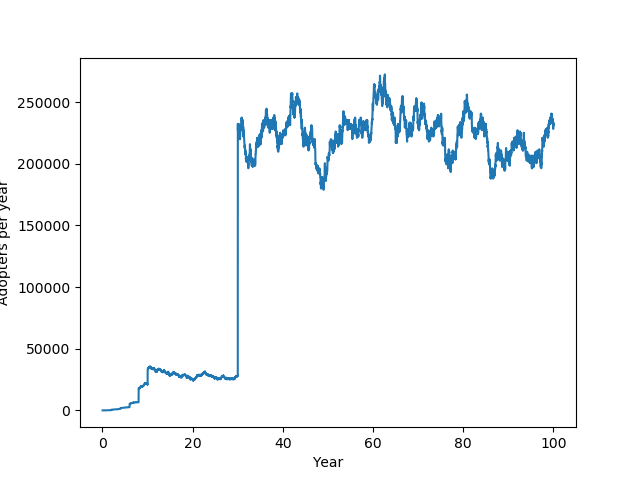
\includegraphics[width=0.5\textwidth]{adopter_per_year}
	\caption{results}
	\label{fig: adopters}
\end{figure}

\begin{figure}\label{fig:emission}
	\centering
	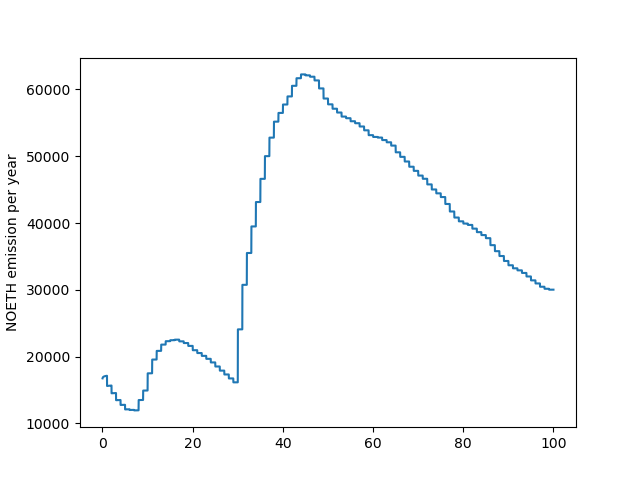
\includegraphics[width=0.5\textwidth]{noth_emission}
	\caption{results}
	\label{fig: noeth_emission}
\end{figure}

\begin{figure}\label{fig:total_circulation}
	\centering
	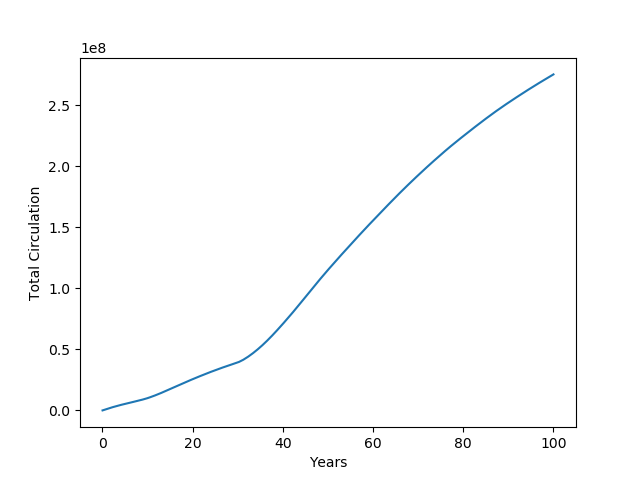
\includegraphics[width=0.5\textwidth]{total_circulation}
	\caption{results}
	\label{fig: total_circulation}
\end{figure}


\begin{thebibliography}{MPP}
	\bibitem[KM]{kermack} Kermack William Ogilvy and McKendrick A. G. \emph{A contribution to the mathematical theory of epidemics}. Proc. R. Soc. Lond. (1927) A115700-721.
	\bibitem[PS]{peruanisibona} Peruani, F. and Sibona, G.  \emph{Reaction processes among self-propelled particles}. Soft Matter (2019), vol. 15, 497.
	\bibitem[V]{verhulst} Verhulst, P.-F.\emph{Recherches math\'ematiques sur la loi d'accroissement de la population}. Nouv. M\'em. Acad. R. Sci. B.-lett. Brux. 18, 1-45 (1845).
\end{thebibliography}
\end{document}